% notes and todo's can be found by searching for ??, @TCC, and @NCM

% For more detailed article preparation guidelines, please see:
% http://f1000research.com/author-guidelines

\documentclass[10pt,a4paper,twocolumn]{article}
\usepackage{f1000_styles}
\usepackage{gensymb}

%% Default: numerical citations
%\usepackage[numbers]{natbib}

%% Uncomment this lines for superscript citations instead
\usepackage[super]{natbib}

%% Uncomment these lines for author-year citations instead
% \usepackage[round]{natbib}
% \let\cite\citep

% Can turn off hyperref if it unwanted, but it is generally useful IMO
\usepackage{xr-hyper}
\usepackage{hyperref}
\usepackage{xcolor}
\hypersetup{
    colorlinks,
    linkcolor={red!50!black},
    citecolor={blue!50!black},
    urlcolor={blue!80!black}
}

%\usepackage{xr} % external refs (for supplemental) (uncomment if not using xr-hyper)
\externaldocument[S:]{supplemental}

\usepackage{nicefrac}
\usepackage{url}
\def\UrlBreaks{\do\/\do-}


\begin{document}

\title{Evaluation of predicted Medfly (\textit{Ceratitis capitata}) quarantine length in the United States utilizing degree-day and agent-based models}
% \titlenote{The title should be detailed enough for someone to know whether the article would be of interest to them, but also concise. Please ensure the broadness and claims within the title are appropriate to the content of the article itself.}

\author[1,2]{Travis C. Collier}
\author[1,3]{Nicholas C. Manoukis}
\affil[1]{Daniel K. Inouye US Pacific Basin Agricultural Research
Center (PBARC), United States Department of Agriculture,
Agricultural Research Service,
Hilo, Hawaii, 96720, USA}
\affil[2]{corresponding author; email: Travis.Collier@ARS.USDA.gov}
\affil[3]{email: Nicholas.Manoukis@ARS.USDA.gov}
% Please list all authors that played a significant role in the research involved in the article. Please provide full affiliation information (including full institutional address, ZIP code and e-mail address) for all authors, and identify who is/are the corresponding author(s).

\maketitle
\thispagestyle{fancy}

\begin{abstract} % max 300 words!
Invasions by pest insects pose a significant threat to agriculture world-wide. In the case of
\emph{Ceratitis capitata} incursions on the US mainland, where it is not officially established,
repeated detections are followed by quarantines and treatments to eliminate the invading population.
However, it is difficult to accurately set quarantine
duration because non-detection may not mean the pest is eliminated.
Most programs extend quarantine lengths past the last fly detection
by calculating the amount of time required for 3 generations to elapse under a thermal unit 
accumulation development model (``degree day''). 
A newer approach is to use an Agent-Based Simulation (ABS) to 
explicitly simulate population demographics and elimination.
Here, predicted quarantine lengths for 11 sites in the continental United States are evaluated
using both approaches.
Results indicate a strong seasonality in quarantine length, 
with longer predictions in the second half of the year compared with the first; 
this pattern is more extreme in degree day predictions compared with ABS.
Geographically, quarantine lengths increased with latitude, though this was 
less pronounced under the ABS.
Variation in quarantine lengths for particular times and places was 
dramatically larger for degree day than ABS,
generally spiking in the middle of the year for degree day 
and peaking in second half of the year for ABS.
Analysis of 34 \emph{C. capitata} quarantines from 1975 to 2017 in California shows that, 
for all but two, quarantines were started in the second half of the year 
when degree day quarantine lengths are longest and have the highest uncertainty.
For a set of hypothetical outbreaks based on these historical quarantines,
the ABS produced significantly shorter quarantines than degree day calculations. 
Overall, ABS quarantine lengths were more consistent than degree day predictions,
avoided unrealistically long values, 
and captured effects of rare events such as cold snaps.
%Results presented here should be useful to program managers and planners preparing for 
%detection and elimination of \emph{C. capitata} in the mainland US.
\end{abstract}

\section*{Keywords}
%Please list up to eight keywords to help readers interested in your article find it more easily.
biosecurity, Mediterranean fruit fly, eradication, invasive pest, agriculture


\clearpage


\section*{Introduction}

Invasions by insects, pathogens and pests are increasingly a 
defining challenge of the 21\textsuperscript{st} century, 
facilitated by global connectivity, climatic shifts, and
other factors\cite{simberloff_impacts_2013,Pimentel2007}, with a particularly 
severe impact on agriculture\cite{paini2016global}.
Invasions by insects that do not become established have a lower public profile
than those that are ``successful'' from the point of view of the insect.
However, there is a greater chance that cases of invasion followed by elimination
will be detected and studied 
when the invading species is of environmental, human health, or 
economic concern\cite{liebhold_population_2008}.
Eradicating local populations of such insects can be desirable and 
feasible\cite{myers_eradication_2000} depending on several factors.

One factor determining the feasibility of elimination
is if the new environment is only marginally or 
seasonally suitable to the invading insect, facilitating its eradication.
Another is when the high cost of allowing establishment leads
to extensive efforts for eradication.
The invasion of the malaria mosquito species \textit{Anopheles gambiae}
into Northeastern Brazil in the 1930's\cite{soper_emphanopheles_1943}
is one example of an invasive insect that was successfully eradicated 
primarily due to the second of these
reasons\cite{causey_ecology_1943,killeen_eradication_2002}.

In the case of \textit{An. gambiae} there have been no reports of
reinvasion, but there are examples of insects that
recurrently invade areas outside their native range and are recurrently
eliminated within relatively few generations.
The Gypsy moth \textit{Lymantria dispar} in Canada\cite{gray_hitchhikers_2010} 
is one such species.
Arguably, another example is 
the screwworm \textit{Cochlyomyia hominivorax} along 
the current northernmost edge of its range in 
Panama\cite{robinson_enabling_2009}
and more recently in Florida\cite{matthews2017news}.

One of the most important instances of repeated invasion 
and elimination by an economically important insect pest is that of 
the Mediterranean fruit fly \textit{Ceratitis capitata} (Wiedemann) (Medfly) 
in California.  
The last four decades have seen a repeated pattern of
invasion, detection, and response 
interspersed by periods of no detections\cite{carey_establishment_1991, papadopoulos_trickle_2013}.
While it has been suggested that this pattern is the result of
cryptic establishment\cite{carey201730}, 
% Though the establishment of these pests is disputed, 
%  a pattern of invasion, detection, and response, 
%  followed by no further detections for a long period, 
%  has been established over the last four decades. 
the majority view is
that Medfly in California is an example of 
a ``metainvasion'', consisting of multiple sequential or
overlapping introductions\cite{davies_bioinvasions_1999}
and repeated eradication\cite{haymer_genetic_1997}.
Still other researchers point to the possibility of different situations
in different regions of the state
\cite{bonizzoni_microsatellite_2001,gasperi_genetic_2002}.
Medfly is occasionally found in 
other parts of the mainland US such as Florida\cite{szyniszewska2016analysis},
and in other countries or areas that are considered 
free of the pest including Eastern Australia, Mexico and Chile\cite{mcinnis2017can}.

The response plan to Medfly in California and the other ``free'' 
regions mentioned above is extensive and costly, 
including a quarantine when detections exceed an established standard
(more than a male or unmated female fly is detected)\cite{gilbert_insect_2013}.
A practical and important problem is how long to maintain 
the countermeasures and quarantine after flies are no longer detected.
Predicting the likely duration of this `post last detection' quarantine period
(hereafter just called quarantine length) would help with
%Predicting the likely duration of required quarantines would help with
management decision-making and planning,
including potential cost savings by having sufficient but not excessive
resources available.

Currently most programs extend quarantine periods past when the last fly is found
by calculating the amount of time required for a given number 
of generations (usually three) to elapse under a thermal unit accumulation (``degree day'')
physiological development model.
Degree day based quarantine lengths have been codified in some legal
regulations, including 
United States Federal code\cite{US-301.32-10},
%(Title 7 Subtitle B Chapter III Part 301.32-10 Treatments),
California\cite{3-CA-ADC-3406}, and Florida.
However, the procedure prescribed only defines when the end of a
quarantine period has been reached after the fact.

For planning and resource allocation, policy makers and managers 
typically attempt to predict the quarantine lengths by using
normal temperatures for forward projection. 
Although it frequently works fairly well,
this approach is mathematically flawed 
and also provides no indication as to the variance or uncertainty
of those predictions.
Even a more rigorous treatment of degree day based values from
historical temperature data can still produce highly variable results
depending on relatively small changes in temperatures or details of
the model formulation\cite{Roltsch1999}, in addition to neglecting
important aspects of the biology.

Recently, another approach to determining effective quarantine 
durations against Medfly via Agent-Based Simulations (ABS)\cite{manoukis_agent-based_2014}
was introduced. 
The MED-FOES system simulates a population of individual Medflies 
under inundative sterile insect technique (SIT) and other controls, 
explicitly modeling elimination as opposed to the degree day 
approach which only determines the time for a specific
number of generations to elapse to estimate quarantine duration.
MED-FOES also allows for the sampling of parameter space
(temperature dependent mortality for each stage, fecundity, etc.)
producing a distribution of possible outcomes.
While an ABS can be arbitrarily complex, MED-FOES is parameterized
in such a way that it can model a `typical' or hypothetical outbreak from only hourly temperature data,
and is therefore similar to degree day methods in its input data requirements.
It is also possible to vary the initial population to model a specific outbreak.

In this paper, predicted quarantine length (PQL) 
for 11 sites in the continental United States were analyzed
(\autoref{fig:sitemap} and \autoref{tab:sites})
based on both the standard thermal accumulation degree day method\cite{ECY:ECY1969503514} 
as well as the MED-FOES ABS\cite{manoukis_computer_2014}. 
Seasonal variation dominates quarantine duration, 
so we aggregated the PQL values for each day of the year 
(Jan.\ 1, Jan.\ 2, etc.) 
across a large number of years (65 for most locations) to produce normals.
This approach enables comparison of the standard degree day 
method to the ABS, but more importantly provides insight 
into seasonal and spatial variations, prediction uncertainties, 
and model reliability.


\begin{figure}[htb!]
\centering
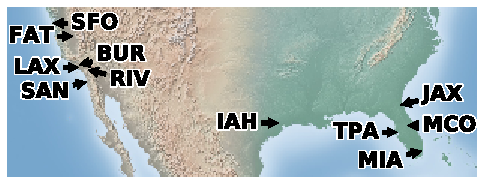
\includegraphics{figs/sitemap.pdf}
\caption{\label{fig:sitemap}Locations of sites analyzed.}
\end{figure}

\begin{table*}[ht!]
\hrule \vspace{0.1cm}
\caption{\label{tab:sites}Weather station (NOAA ISD) sites used.}
\centering
\begin{tabledata}{llllrrrl}
\header Callsign & Station Name (as shown in data records) & State & Latitude & Longitude & Elevation & Start year \\
\row KSFO &  SAN FRANCISCO INTERNATIONAL A &  CA &  +37.620 &  -122.365 &  2.4 & 1950 \\
\row KFAT &  FRESNO YOSEMITE INTERNATIONAL &  CA &  +36.780 &  -119.719 &  101.5 & 1950 \\
\row KBUR &     BURBANK-GLENDALE-PASA ARPT &  CA &  +34.201 &  -118.358 &  236.2 & 1973 \\
\row KLAX &  LOS ANGELES INTERNATIONAL AIR &  CA &  +33.938 &  -118.389 &  29.6 & 1950 \\
\row KRIV &         MARCH AIR RESERVE BASE &  CA &  +33.900 &  -117.250 &  468.2 & 1950 \\
\row KSAN &  SAN DIEGO INTERNATIONAL AIRPO &  CA &  +32.734 &  -117.183 &  4.6 & 1950 \\
\row KJAX &  JACKSONVILLE  INTERNATIONAL A &  FL &  +30.495 &  -81.694 &  7.9 & 1950 \\
\row KIAH &  G BUSH INTERCONTINENTAL AP/HO &  TX &  +29.980 &  -95.360 &  29.0 & 1970 \\
\row KMCO &  ORLANDO INTERNATIONAL AIRPORT &  FL &  +28.434 &  -81.325 &  27.4 & 1973 \\
\row KTPA &    TAMPA INTERNATIONAL AIRPORT &  FL &  +27.962 &  -82.540 &  5.8 & 1950 \\
\row KMIA &    MIAMI INTERNATIONAL AIRPORT &  FL &  +25.791 &  -80.316 &  8.8 & 1950 \\
\end{tabledata}
\end{table*}


\section*{Methods}

\subsection*{Sites and Temperature Data}
Hourly air temperature data for 11 sites was downloaded from 
NOAA's Integrated Surface Database (ISD) dataset\cite{smith_integrated_2011,NOAA_ISD_portal}.
The airport sites shown in \autoref{fig:sitemap} 
were chosen for their biological relevance and 
availability of high quality hourly data over a long time frame.

Sites are referred to here by the last three letters of the callsign shown in 
\autoref{tab:sites}.
For 8 sites (SFO, FAT, LAX, RIV, SAN, JAX, TPA, and MIA), temperature data starting on 1950-01-01 was used.
The 3 other sites contained large (${>}14$ days) gaps or other problems in the early years of their data,
so data starting on 1970-01-01 for IAH and 1973-01-01 for BUR and MCO was used.
For all sites, temperature data from the start date through 2017-05-15 was used
to generate PQLs for dates ranging from the start date to 2016-01-01.

Data was fetched and parsed using the \texttt{Fetching and parsing ISH.ipynb} program.
Records for the same station callsign were merged, since identification, format, 
and precise location of stations has changed over time.
The data was then cleaned using the 
\texttt{Cleaning temperatures.ipynb} program by 
removing outliers, 
identifying large gaps ($>$ 3 hours), 
resampling to every hour on the hour using linear interpolation,
and filling the large gaps using day-over-day linear interpolation
(interpolating using values for the same hour of day from previous and following days).
The processing programs and resulting temperature datasets are 
provided in the Supplemental Materials.


\subsection*{Degree-Day Calculation}
Degree-days were computed by the single-sine method\cite{ECY:ECY1969503514}
using a base development temperature of 12.39\degree C (53.3\degree F) 
and 345.56 degree-days Celsius (DDc; 622 DDf) per generation 
following the standard set by California Department of Food and Agriculture
regulation 3406(b)\cite{3-CA-ADC-3406,CDFA_Medfly}.
%single-triangle\cite{10.2307/1933072}
Since hourly temperature data are available, 
we also calculated degree-days by simple summation
for comparison\cite{Roltsch1999}.
For each date, the number of days required for 3 generations of degree-day 
based life cycles was computed.
These calculations are implemented in \texttt{Temperature functions.ipynb} in the Supplemental Materials.


\subsection*{Agent-based Simulations: MED-FOES}

MED-FOES\cite{manoukis_agent-based_2014,manoukis_computer_2014} is 
an agent-based simulation explicitly modeling the eradication of a population of Medflies 
under inundative sterile male releases (sterile insect technique or SIT) and other interventions
such as increased trapping and foliar sprays.
A MED-FOES simulation models a single non-spatial population starting from a given population size and age distribution 
tracking the number of individuals through time until the last 
fly (Agent) dies and the population is eliminated.
In addition to hourly temperatures, simulation parameters include: 
the initial population, 
additional mortality induced by control efforts,
the effectiveness of SIT, 
and a large number of biological parameters for which ranges are known from 
the literature including temperature-dependent development and mortality.
The simulations were performed using the same hourly time series of temperature values 
used for degree-day calculations.

Due to the fact that many of the parameters are only known to within a range,
2500 individual MED-FOES simulations were run for each start date at each site 
evenly sampling different regions of parameter-space via the 
Latin Hypercube Sampling\cite{10.2307/1403510} procedure.
This set of simulations, encompassing a range of possible elimination outcomes, is referred to as a `run'.
%simulation -> run -> runset is the terminology I've been using
The number of days from the start date required for
95\% of the simulations in a run to be eliminated is 
taken as a conservative prediction of needed quarantine length and referred to as 
ABS PQL\cite{manoukis_agent-based_2014}.

Varying the start date for different simulations was achieved by simply 
starting at different points in the input temperature file; 
for this study a run starting every 7 days over the range of dates available for each site.
Each set of runs for a single site over a range of starting dates is referred to as a `runset'.
All runsets were conducted with the same input parameters aside from temperature.
Initial population numbers were chosen as a ``standard outbreak'' based on seven real 
outbreaks modeled previously\cite{manoukis_agent-based_2014}.
The 7 day interval ABS PQL values were upsampled to daily values using linear interpolation
to allow day-of-year aggregations across years and comparisons with daily degree day based PQLs.

MED-FOES version 0.6.2 was run under
Open Grid Scheduler/Grid Engine 2011.11 on a CentOS 6.6 HPC cluster.
The MED-FOES code, configuration files, and helper scripts are provided in the Supplemental Materials.
Overall, we created 11 runsets (one for each site), 
each containing runs starting every 7 days over the input temperature data range for that site,
where each run contained 2500 individual simulations sampling different regions of 
biologically plausible parameter space; 
a total of approximately $86{\times}10^6$ simulations.


\subsection*{Statistical analysis}

The main results reported here are `normals' in a meteorological sense of the term,
but without the typical running mean smoothing which would complicate
interpretation.
For a variable of interest (eg.\@ temperature or PQL), 
all values for the same calendar day irrespective of year (eg.\@ 20-July) are
aggregated and summary statistics such as mean, minimum, maximum, and standard deviation 
are computed for each aggregation.
\texttt{Temperature functions.ipynb} contains the code used to perform normal calculations, 
and the code generating figures as well as all statistical analysis 
is \texttt{Summary Figures.ipynb}
(Jupyter Notebook\cite{PER-GRA:2007}, module and version information documented in the file).

The results reported here are the normals of PQL computed using the full temperature time series
as opposed to computing PQL from the normal of the temperature timeseries.
While the latter is fairly common practice, it is not mathematically proper 
since, as with means, the normal of a function of $X$ is not generally equal to the function applied to the normal of $X$.
Additionally, by computing the normals of the predicted quarantine durations, 
we can investigate properties of the distribution of values as shown in 
\autoref{fig:DD_variation_summary} and \autoref{fig:pe95_variation_summary} 
and the ``supernorm" supplemental figures 
S\ref{S:fig:temperature_supernorm}, 
S\ref{S:fig:ddPQL_supernorm},
and S\ref{S:fig:medfoesPQL_supernorm}.

%\subsection*{Historical quarantines}
%
%%\begin{figure}[ht!]
%%\centering
%%\includegraphics[width=0.4\textwidth]{figs/fig_historic_quarantines.pdf}
%%\caption{\label{fig:historic_quarantines}
%%Day-of-year timing and size of historic Medfly quarantines in CA.
%%SFO 1980 and LAX 1991 were very long duration outliers.
%%Quarantines before the preventative release program was initiated in 1994 are denoted by `X's.
%%}
%%\end{figure}
%
%A list of 34 Medfly quarantines in CA dating from 1975 to early 2017 was obtained from 
%APHIS\cite{??}.  
%Each quarantine location was associated with a site from the 11 sites analyzed here.
%For a number of the historic quarantines, this is a rough association since temperature/climate
%can vary significantly over a short distance, especially between coastal and more 
%inland locations.
%Temperature data from the nearest site and the historic quarantine start date was used to 
%compute the 3 generation degree-day duration along with MED-FOES 95\% elimination.
%PQLs were also computed using the day-of-year of the historic quarantines 
%and the mean of the normal PQL values for the nearest site.
%Values are reported in the supplemental table ??.
%%\ref{fig:historic_quarantines}


\section*{Results}

\begin{figure*}[htp!] % could add 'p' placement to allow it to be on its own page
\centering
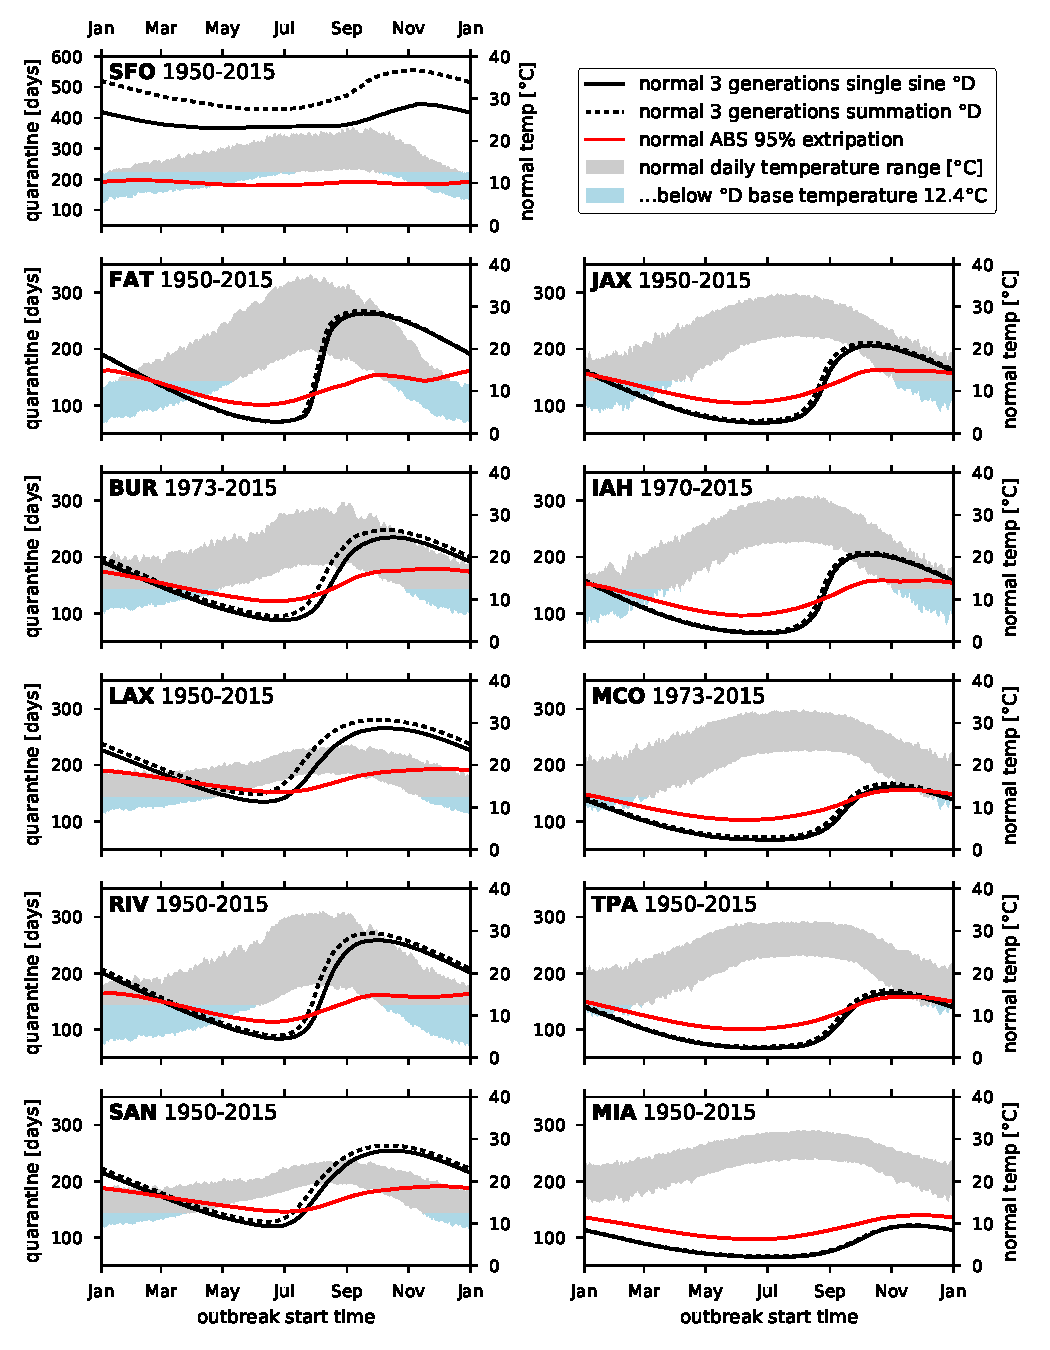
\includegraphics{figs/fig_main.pdf}
\caption{\label{fig:main_summary}Summary of normal predicted quarantine length 
for each site and start date (last fly detection).
Year range of input temperature data used is inclusive.
All panels have identical limits except SFO quarantine.}
\end{figure*}

\begin{figure*}[ht!]
\centering
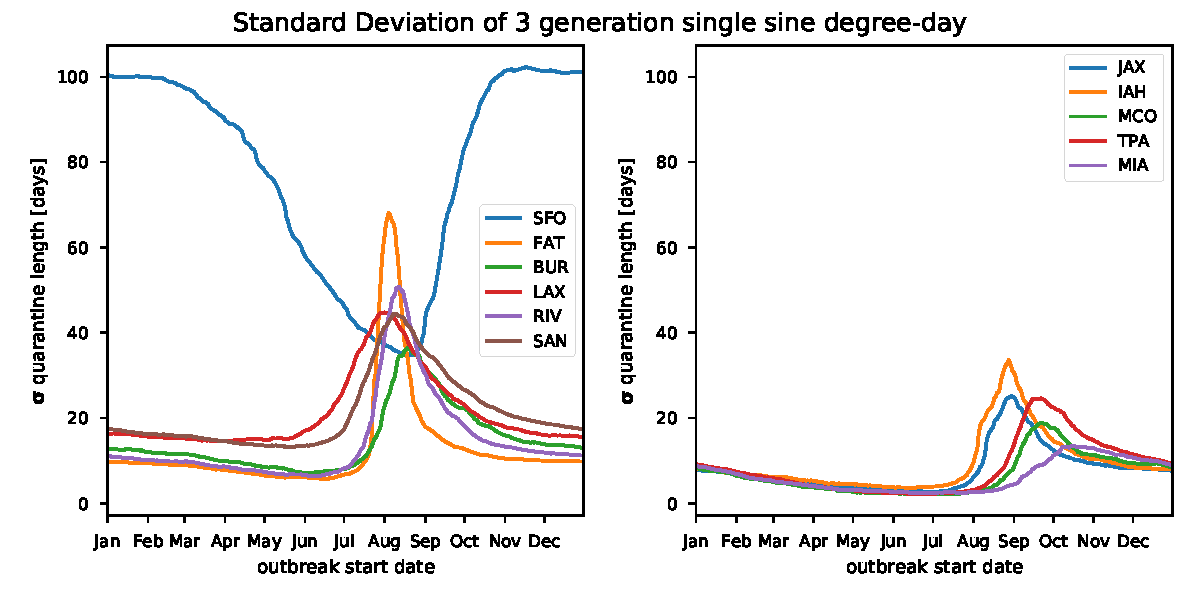
\includegraphics{figs/fig_BMDD_variation.pdf}
\caption{\label{fig:DD_variation_summary}Variation in predicted quarantine length
for each site and start date
based on 3 generations of single-sine degree day accumulation.}
\end{figure*}

\begin{figure*}[ht!]
\centering
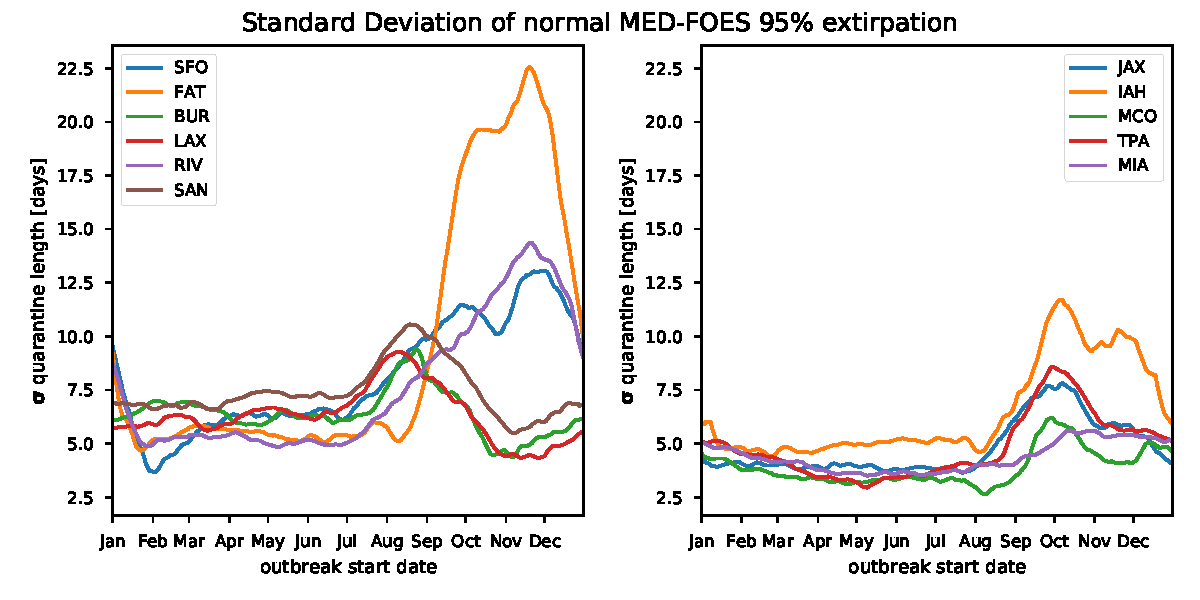
\includegraphics{figs/fig_pe95_variation.pdf}
\caption{\label{fig:pe95_variation_summary}Variation in predicted quarantine length 
for each site and start date
based on 95\% of MED-FOES agent-based simulations showing elimination.}
\end{figure*}


\autoref{fig:main_summary} shows 
the mean of the normal PQL based on 3 generation degree day accumulation 
and MED-FOES 95\% elimination
along with the minimum and maximum of the normals for temperatures.
\autoref{fig:DD_variation_summary} and \autoref{fig:pe95_variation_summary} show the 
standard deviations ($\sigma$) of the normals for the degree day and ABS based PQL.

There is significant variation in PQL across both time and location.
The temporal variation in PQL is dominated by a yearly cycle, 
characterized by the normal values shown in \autoref{fig:main_summary}.
\autoref{tab:variance_captured_by_normal} shows the percentage of variance in 
quarantine length predictions captured by the mean of the normal yearly cycle ($R^2$) for each site.
At all but one site, greater than 75\% of the variance in both degree day and ABS based PQLs
is accounted for by the mean normal, and the majority exceed 90\%.
SFO is an exception to this common trend, with the mean normal accounting for only 9.1\% of the variation in 
degree day based PQL and 28.0\% of the ABS based PQL.
This is also reflected in supplemental figures
S\ref{S:fig:ddPQL_supernorm},
and S\ref{S:fig:medfoesPQL_supernorm}.

\begin{table}[htb!]
\hrule \vspace{0.1cm}
\caption{\label{tab:variance_captured_by_normal}
Percentage of PQL variance captured by the mean of the normal.  
DD PQL is the 3 generation single sine degree day based prediction, 
and ABS PQL is the MED-FOES agent-based simulation predictions.}
\centering
\begin{tabledata}{lrr}
%\header & \multicolumn{2}{c}{$R^2$} \\
\header Site & DD PQL $R^2$ & ABS PQL $R^2$\\
\row SFO &   9.12\% & 28.01\% \\
\row FAT &  93.93\% & 75.68\% \\
\row BUR &  90.71\% & 90.88\% \\
\row LAX &  80.17\% & 83.07\% \\
\row RIV &  92.23\% & 81.89\% \\
\row SAN &  80.99\% & 80.91\% \\
\row JAX &  96.45\% & 94.78\% \\
\row IAH &  95.10\% & 91.80\% \\
\row MCO &  94.62\% & 95.77\% \\
\row TPA &  91.91\% & 94.40\% \\
\row MIA &  88.42\% & 92.00\% \\
\end{tabledata}
\end{table}


\subsection*{Seasonal dependence}

Seasonal variation, evidenced by the general shape of the curves shown in \autoref{fig:main_summary}, 
is doubtless familiar to anyone engaged in Medfly pest management.
Outbreaks starting in the late summer, autumn, or early winter will extend through relatively cold periods,
when thermal dependent development will be slow and therefore extend the duration of quarantine required
for 3 generations of degree days to accumulate (referred to as DD PQL hereafter).
Similarly, outbreaks starting in the spring or early summer often lead to short quarantines due
to the relatively high temperatures.

This familiar pattern is also seen in the ABS PQLs despite it being 
quite different in nature from simple degree day accumulation.
However, the ABS predictions show a smaller seasonal swing.
The ABS generally produces a smaller overall range of PQLs,
with longer quarantines than DD PQL for spring and early summer outbreaks,
and shorter quarantines for late summer through early winter in almost all cases.

A particular feature of interest, shown most dramatically at FAT in \autoref{fig:main_summary},
is that ABS PQL often flattens out or even dips for quarantines starting in the late 
autumn or early winter.  This can be due to relatively rare and brief cold-snaps,
normally lasting only a few hours, which increase mortality.
Since DD PQL does not account for mortality, it misses the effect of cold-snaps entirely.
This effect is most clearly seen at more northern and 
inland sites where cold-snaps are more likely: 
particularly FAT and RIV, but also BUR, LAX, JAX, and IAH.

\subsection*{Geographic dependence}

\begin{figure*}[ht!]
\centering
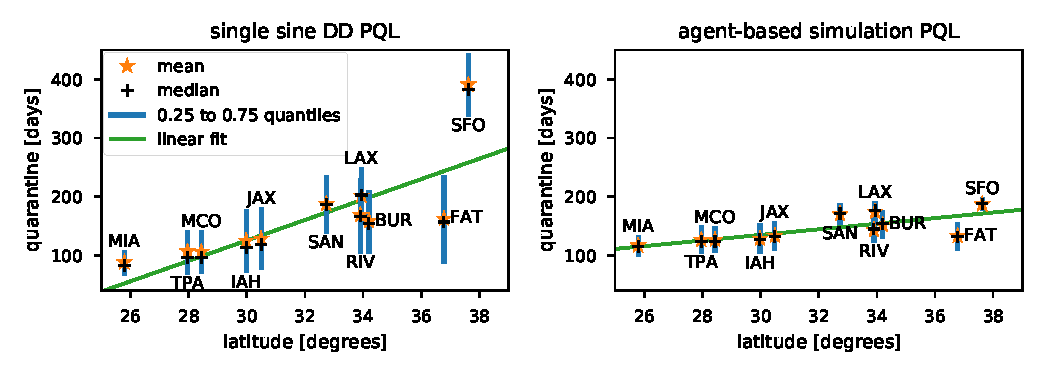
\includegraphics{figs/fig_latitude_trend_withSFO.pdf}
\caption{\label{fig:latitude_trend} Predicted quarantine length dependence on latitude.
For each site, the mean, median, and inter-quartile range are shown (similar to a boxplot).
An ordinary least-squares linear fit to the median values is shown by the green lines.
The left pane is for single sine degree day predictions,
and MED-FOES ABS based predictions are in the right pane.
}
\end{figure*}

PQL generally shows a positive correlation with latitude, and 
sites are ordered by latitude in the figures and tables here.
As seen in \autoref{fig:main_summary}, higher latitude sites tend to have longer PQLs
as well as larger seasonal swings for both degree day and ABS based predictions.

\autoref{fig:latitude_trend} shows the relationship between PQL and latitude.
An ordinary least squares fit to the median PQL at each site shows a significant slope for
both DD PQL ($F{=}14.08$, $p{=}0.005$) and ABS PQL ($F{=}10.55$, $p{=}0.010$), but
the degree day based predictions are more sensitive to latitude than the ABS
(coefficients of 17.39 and 4.78 respectively).
Additionally, the ABS predictions are more stable for SFO, and to a lesser extent FAT, 
where the degree day model for Medfly produced PQLs that appear either unrealistically long (SFO) 
or are subject to rapid and extreme seasonal variation in the mid year (FAT).

In addition to the variation associated with latitude, 
large differences in PQLs computed for the same start date
can exist between even relatively nearby sites.
For example, the differences in both degree day and ABS PQLs 
for the three sites in the Los Angeles region (LAX, BUR, RIV) 
(shown in the supplemental figure S\ref{S:fig:PQL_difference_between_sites_LA})
display a strong seasonal component with a spike in July and/or August.
The difference in DD PQL between LAX and BUR is normally about a month
(overall median=35 days; overall 25\% \& 75\% quantiles are 28 \& 45 days), 
but the median difference of the normal exceeds 75 days in August with some 
PQL differences up to 142 days.
Differences in ABS PQLs are more seasonally stable, 
with the LAX minus BUR difference not exceeding 42 days
for any start date in the 43 years analyzed here.


\subsection*{Variance and uncertainty}

\autoref{fig:DD_variation_summary} and \autoref{fig:pe95_variation_summary}
report the standard deviation ($\sigma$) of the normal for DD PQL and the MED-FOES ABS PQL 
respectively.
These indicate the year to year variability of the PQL for outbreaks starting at a
given time of the year and can be used to gauge the uncertainty of predictions based on 
past PQLs relative to the actual quarantine length which will be required.
Similar information is represented by the inter-quartile ranges 
shown in \autoref{fig:latitude_trend} and supplemental figures
S\ref{S:fig:ddPQL_supernorm},
and S\ref{S:fig:medfoesPQL_supernorm}.
The distributions of PQL values for a site and day-of-year (aggregating across years) 
are generally not highly skewed, making $\sigma$ a relatively easy to interpret measure of uncertainty.

Excluding SFO, the mean normal is a good predictor of DD PQL with $\sigma$ values below 20 days
except for the late summer and early autumn, where variance increases 
due to quarantines extending through the cold season.
FAT and, to a lesser extent, RIV show this increase more dramatically, presumably due to their more 
arid/inland climates where both daily and seasonal temperature ranges are larger
(also see \autoref{fig:main_summary}).
The standard deviation generally decreases with decreasing latitude, together with reduced means.
The standard deviation in DD PQL for SFO shows an inversion of the seasonal trend 
other sites exhibit.
This is due to the colder temperatures leading to extremely long DD PQLs, 
frequently extending across two winter seasons.

The standard deviations of the ABS PQL normals 
shown in \autoref{fig:pe95_variation_summary}
are generally about \nicefrac{1}{2} as large as for DD PQL.
This indicates that the ABS PQL not only shows less dramatic seasonal swings, 
but is also produces more consistent predictions across years.
Values again generally decrease with latitude, but less consistently than DD PQL $\sigma$ of normals.
Also, unlike with the DD PQL, the results for SFO appear consistent with other sites.

A notable feature is that BUR, LAX, and SAN all show an increase in the year to year variation
in ABS PQLs starting in July and extending through November, 
while that increase for all other sites starts in July or August 
but extends to January or February.
Additionally, results for FAT show a sharp increase in uncertainty starting in September, fitting with the 
more arid/inland climate.  RIV shows a significant but more gradual increase.

\subsection*{Historical quarantines}

Thirty-four Medfly quarantines in CA dating from 1975 to early 2017 were analyzed
(supplemental table S\ref{S:tab:historical_quarantines}).
The start of all but two of these quarantines was in the latter half of the year
(July through December) when DD PQLs are typically relatively long,
with 68\% ($23/34$) occurring in September through October when DD PQLs are
longest. 
August, the month where uncertainty in DD PQL often spikes 
(see \autoref{fig:DD_variation_summary}), 
accounts for 30\% ($7/34$) of historic quarantines.

For each historic quarantine start date, the DD PQL and ABS PQL 
for the closest of the 11 sites analyzed above (see \autoref{fig:sitemap} and \autoref{tab:sites}) 
to the actual outbreak location was determined
(see supplemental table S\ref{S:tab:historical_quarantines}).
For this set of hypothetical quarantines, 
the ABS produced significantly shorter quarantines
(mean=169.7 days, $\sigma$=21.8 days)
than simple 3 generation degree day accumulation
(mean=234.2 days, $\sigma$=79.2 days)
(\textit{df}=33, $t{=}6.01$, $p{<}10^{-5}$).
Additionally, the variance in the difference between quarantine lengths
using a specific date and the mean of the normal PQL for that day of year
was smaller for the ABS ($\sigma$=8.2 days)
than with degree day ($\sigma$=25.9 days)
(\textit{df}=33, $F{=}9.92$, $p{<}10^{-8}$).


% @ TCC Maybe for supplemental...
%\begin{table}[htb!]
%\hrule \vspace{0.1cm}
%\caption{\label{tab:histoirc_quarantine_PQL}
%}
%\centering
%\begin{tabledata}{lrrr}
%\header & 
%\vtop{\hbox{\strut DD PQL $-$}\hbox{\strut normal}} &
%\vtop{\hbox{\strut ABS PQL $-$}\hbox{\strut normal}} &
%\vtop{\hbox{\strut DD PQL $-$}\hbox{\strut ABS PQL}} \\
%%\header & DD PQL - normal & ABS PQL - normal & DD PQL - ABS PQL\\
%\header & \multicolumn{3}{c}{[days]} \\
%\row N        & 34    & 34    & 34    \\
%\row mean     & -6.4  & -0.6  & 64.5  \\
%\row $\sigma$ & 25.9  & 8.2   & 62.6  \\
%\row min      & -77.7 & -22.9 & -40.1 \\
%\row 25\%     & -17.5 & -2.7  & 39.0  \\
%\row 50\%     & -4.7  & -0.5  & 67.0  \\
%\row 75\%     & 11.5  & 3.3   & 93.6  \\
%\row max      & 36.1  & 16.4  & 191.8 \\
%\end{tabledata}
%\end{table}




\section*{Discussion}
% The discussion should include the implications of the article results in view of prior work in this field.

The principal contributions of this work can be broken down into three categories: 
1) Comparison of PQLs as determined by the degree day and ABS methods. 
2) variation in average PQLs across time of year and space, and
3) variation in PQLs within a time of year and location.
Consideration of all three of these by program managers, planners and other decision makers 
is likely to
improve management of Medfly outbreaks %@NCM: is this OK?
by informing resource allocation ahead of outbreaks, reducing 
quarantine costs in some cases, and reducing risk from premature quarantine suspension in others. 
The results presented cover most of the latitudinal range 
of Medfly suitability within the United States 
as well as many sites of probable introduction,
and will hopefully find use as a general guide.

% overall comparison of DD and ABD PQLs here.

Eradication models are extremely difficult to test for accuracy given 
the impracticality of experimental introductions and 
the sparse and idiosyncratic nature of historic outbreaks.
However, analyzing the timing and locations of historic outbreaks 
suggests that quarantine lengths would generally be more consistent
and shorter on average in California if estimated by ABS compared with degree day. 

Requiring a fixed number (typically 3) generations of degree days to pass is 
a ``tried and true" method, but not explicitly an extirpation model.
It may overestimate required quarantine length through cold weather\cite{manoukis_agent-based_2014}
and may underestimate length when growth conditions are very favorable, 
which somewhat paradoxically leads to shorter degree day based quarantine periods after the 
last fly detection since generation times are shorter. %@TCC|@NCM CITE??
%However, the simplicity of degree day and the "has worked so far" nature
%means it will likely continue to be the regulatory benchmark.
However, the simplicity of the degree day calculation is a point in its favor, together with 
its record of generally avoiding subsequent detections after
eradication measures and quarantine establishment\cite{mcinnis2017can}.

ABS results may be used to inform and modulate responses and treatments such as
delimination trapping, fruit sampling, and eradication measures which are under
the some discretion of managers.
In situations where DD PQL greatly exceed those from the ABS, it is likely
that degree day is missing important effects, such as cold snaps, which may justify
shortening quarantine periods.
On the other hand, in cases where the ABS predicts longer times to elimination, it
is plausible that the degree day indicated quarantine is optimistically short, and 
eradication treatments and SIT releases should be conducted even more aggressively than
normal to ensure eradication is achieved within the degree day based period. %@NCM check this sentence please


A few specific results arising from overall comparisons of different locations are worth highlighting. 
In general, DD PQLs for Medfly 
generated from San Francisco International Airport temperature data
 are almost certainly too long for the entire year.
The ABS PQLs are flatter and seem more realistic at around 200 days for San
Francisco compared with the 400-550 days of DD PQLs. 
For several other California locations (typified by Fresno and 
Riverside) DD PQLs are in close alignment with those from the ABS 
for the first half of the year 
but go significantly longer in the cooler months. 
For three of the four Florida locations analyzed, 
DD PQLs are significantly shorter than the ABS results
 (Miami, Tampa, and Orlando).
The extent of the difference in those Florida locations is smaller in the later months of the year,
but the generality of this pattern suggests that the margin of safety for quarantines as 
calculated by degree day in those locations may be smaller than expected. 

% @NCM --
% Other systematic comparisons of (PQLs? development?) include .. (PLUG Davis paper here) 
% Are there other papers we should compare with here? I would guess yes...

There is significant variation in PQL depending on the location of the outbreak, 
with the extremes in our study sites represented by Miami and San Francisco.
These geographic results could be
%compared directly to previous efforts to model climatic suitability of different parts of the US 
%for Medfly, by equating longer PQLs with higher climatic suitability.
% @NCM... Actually, it can't.  High suitability normally means high reproduction rate => fast generations => low PQL.  That is the paradox thing I mentioned. --@TCC
compared to previous efforts to model climatic suitability of different parts of the US.
One of the early studies on the subject focused on Medfly found higher climatic suitability in 
Florida locations (Fort Pierce and Orlando) compared with California 
sites\cite{messenger_bioclimatic_1954}. 
Within California, however, those authors found a higher number of suitable months in coastal 
areas such as Oceanside compared with Riverside and Fresno, roughly paralleling our 
findings (compare Los Angeles or San Diego with Fresno or Riverside).
A more recent analysis of climatic suitability likewise concludes that coastal 
S. California is the most favorable area of the state for Medfly, but 
favorability drops inland in the south due to desert conditions.
Suitability in central and northern California is limited by cold temperatures and 
freezes\cite{gutierrez_assessing_2011}. 


% @NCM... I can't think of anything clever to say here.  It pretty much follows what everyone already knows.  Feel free to add something though  --@TCC
% Seasonal variation within locations revealed WORDS ON SEASONAL HERE
% A ref which points to more: Anna's 2014 paper; refs she cites "It is well documented in regional studies from several areas of the world that Medfly has a highly seasonal pattern to its population dynamics"...:
% https://www.ncbi.nlm.nih.gov/pmc/articles/PMC4222914/


% variation within location/time
An important aspect of ABS PQLs is variation within particular times of years and locations. 
Rare events like cold snaps can increase mortality in the ABS,
and thereby lead to shorter PQLs than expected based on historical averages, or DD PQLs.
The specificity of the ABS is helpful for determining 
when quarantines might be safely suspended due to a rare event,
something that might not be captured by the degree day model.
The degree day model includes only development for generating PQLs,
and development is halted at low temperatures, extending quarantine lengths.
The ABS, however, also includes mortality for generating PQLs,
which means that low temperatures can significantly reduce estimates.
% perhaps name names of locations
% where the variation is particularly acute (like FAT?)
% Possibly put a paragraph on variation in PQLs seen in figs 3,4- patterns different for ABS vs DD (This is touched on below with the uncertainty stuff.)

Historically in California, quarantines have most frequently occurred at times of year when 
degree day based quarantines are drawn out by cold weather and the MED-FOES ABS model predicts significantly
shorter durations.
Furthermore, 30\% of those historic quarantines happened in August where there is a great 
deal of uncertainty in forward predictions of degree day quarantine durations based on normal values.
If we assume those historic CA quarantines are a guide, the ABS model would very likely
produced more predictable and shorter quarantine durations for future outbreaks.



%%%%%

%By expanding on previous work\cite{manoukis_agent-based_2014}, this study suggests that an 
%improved approach to setting quarantine lengths would 
%include estimates from the DD method and from the ABS.
Combination of the two methods analyzed here could leverage the best aspects of both methods for 
determining optimal quarantine length. 
The initial quarantine length estimate could be quickly produced via degree-day calculation
or the ABS
based on the distribution of PQL values generated using historical temperatures.
This would generate not just a single ``typical'' value as the current method of projecting
using historical average/normal temperatures does, 
but a range of outcomes.
The median ``most likely'' value may be used for official estimates, while
the variance and extremes would provide managers and affected parties additional
information vital for planning.

Once the three generation period has started after the last fly find, weekly ABS simulations
could indicate the likelihood that the pest has been successfully eliminated.
If a threshold of 95\% of simulations show elimination, 
the decision to end quarantine early could be made, 
or in the case where the ABS has not reached the 95\% threshold at the end of the DD PQL 
additional measures could be considered to reduce the risk of re-detection.
% @NCM... What do you think about adding something like...
%However, the choice of 95\% as the threshold is somewhat arbitrary and does not 
%directly represent a probability of a quarantine being successful.  In fact, it is most likely 
%overly conservative, since that 5\% of persisting simulations are the worst possible combination of
%plausible parameter values (high reproduction rate, low mortality, etc.)
%The precise choice of threshold value may be a useful point of adjustment for policymakers.

% @NCM|@TCC... Some line(s) with a final overall conclusion?


%\section*{Conclusions}
%Please state what you think are the main conclusions that can be realistically drawn from the findings in the paper, taking care not to make claims that cannot be supported.


\subsection*{Author contributions}
NCM: Devised and wrote the MED-FOES ABS.
TCC: Produced figures and wrote the temperature parsing, degree day, and analysis code.
Authors contributed equally to manuscript.
%In order to give appropriate credit to each author of an article, the individual
%contributions of each author to the manuscript should be detailed in this section. We
%recommend using author initials and then stating briefly how they contributed.

\subsection*{Competing interests}
None to declare.

\subsection*{Grant information}
This research was funded by USDA-ARS, project number 2040-22430-025-00D and by the Headquarters 
Research Associate program (TCC).

\subsection*{Acknowledgements}
We thank J. Hendrichs, S. Gieb, S. Sim, and T. Fezza 
for comments on an early draft of this paper, 
and N. Mullaly (USDA-APHIS) for data on historical outbreaks. 
This work was supported by the US Department of Agriculture, Agricultural Research Service. Opinions, findings, conclusions or recommendations expressed in this publication are those of the authors and do not necessarily reflect the views of the USDA. USDA is an equal opportunity provider and employer.

{\small\bibliographystyle{unsrtnat}
\bibliography{main}}

% \bigskip
% References can be listed in any standard referencing style that uses a numbering system
% (i.e. not Harvard referencing style), and should be consistent between references within
% a given article.

% Reference management systems such as Zotero provide options for exporting bibliographies as Bib\TeX{} files. Bib\TeX{} is a bibliographic tool that is used with \LaTeX{} to help organize the user's references and create a bibliography. This template contains an example of such a file, \texttt{sample.bib}, which can be replaced with your own. Use the \verb|\cite| command  to create in-text citations, like this\cite{Smith:2012qr} and this\cite{Smith:2013jd}.


% See this guide for more information on BibTeX:
% http://libguides.mit.edu/content.php?pid=55482&sid=406343

% For more author guidance please see:
% http://f1000research.com/author-guidelines


% When all authors are happy with the paper, use the 
% ‘Submit to F1000Research' button from the menu above
% to submit directly to the open life science journal F1000Research.

% Please note that this template results in a draft pre-submission PDF document.
% Articles will be professionally typeset when accepted for publication.

% We hope you find the F1000Research Overleaf template useful,
% please let us know if you have any feedback using the help menu above.


\end{document}
